\documentclass[12pt]{article}
 
\usepackage[margin=1in]{geometry} 
\usepackage{amsmath,amsthm,amssymb}
\usepackage{hyperref}
\usepackage{graphicx}
\usepackage{xcolor}
\usepackage[many]{tcolorbox}
\tcbuselibrary{listings}
\usepackage{listings}
\usepackage{float}
\usepackage{hyperref}

\definecolor{lg}{HTML}{f0f0f0}

\newtcblisting{pycode}{
    colback=lg,
    boxrule=0pt,
    arc=0pt,
    outer arc=0pt,
    top=0pt,
    bottom=0pt,
    colframe=white,
    listing only,
    left=15.5pt,
    enhanced,
    listing options={
        basicstyle=\small\ttfamily,
        keywordstyle=\color{blue},
        language=Python,
        showstringspaces=false,
        tabsize=2,
        numbers=left,
        breaklines=true
    },
    overlay={
        \fill[gray!30]
        ([xshift=-3pt]frame.south west)
        rectangle
        ([xshift=11.5pt]frame.north west);
    }
}

\lstset{
    language=Python,
    basicstyle=\small\ttfamily,
}

 
\begin{document}
 
\title{Exercise 5}
\author{Cristian Manuel Abrante Dorta - 888248\\
ELEC-E8125 - Reinforcement Learning}

\maketitle
\section{Policy gradient}

\subsection{Task 1}
\textbf{Implement policy gradient for the CartPole environment with continuous
action space.}\\

The implementation of the policy gradient algorithm with $\sigma^2 = 5$, gave the following plot of result:

\begin{figure}[ht]
    \centering
   \begin{minipage}{0.33\textwidth}
     \centering
     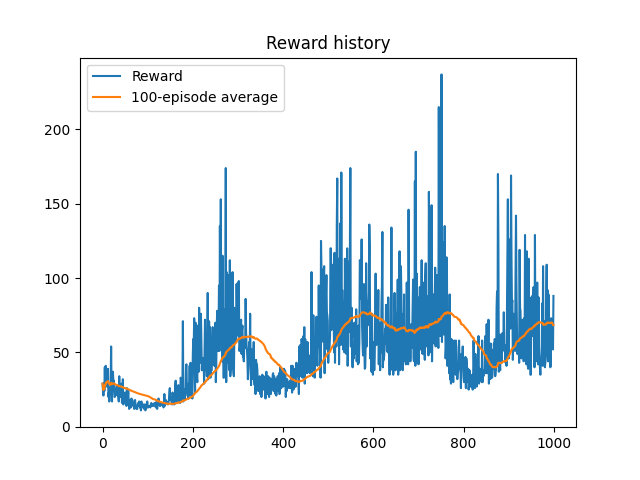
\includegraphics[width=0.9\linewidth]{exercise-5/plots/task-1a.png}
     \caption{Basic REINFORCE without baseline}
     \label{fig:task-2-1}
   \end{minipage}\hfill
   \begin{minipage}{0.33\textwidth}
     \centering
     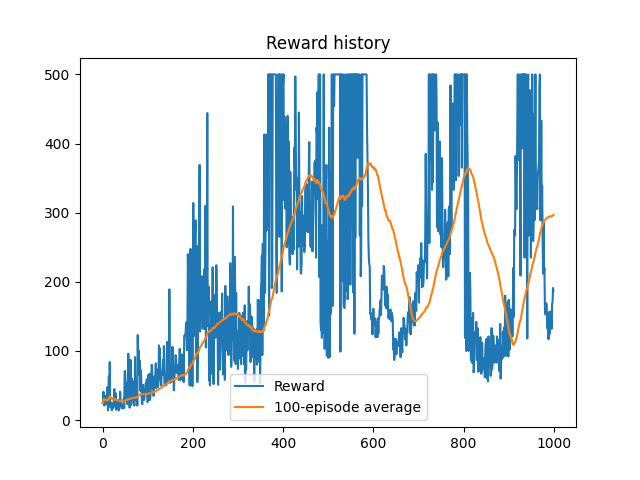
\includegraphics[width=0.9\linewidth]{exercise-5/plots/task-1b.png}
     \caption{REINFORCE with $b=20$}
     \label{fig:task-2-1}
   \end{minipage}\hfill
   \begin{minipage}{0.33\textwidth}
     \centering
     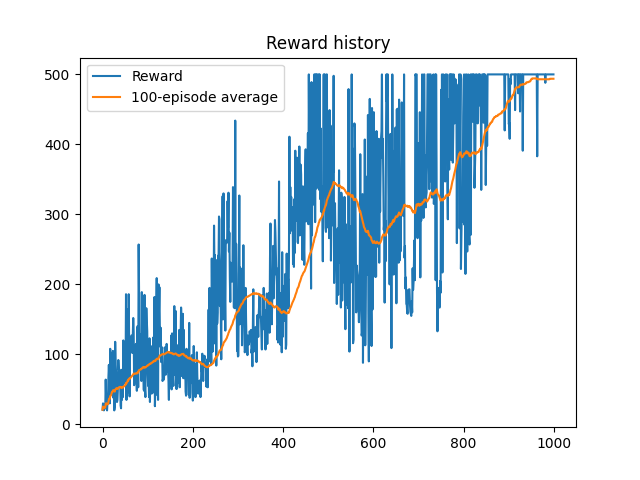
\includegraphics[width=0.9\linewidth]{exercise-5/plots/task-1c.png}
     \caption{REINFORCE with normalized rewards}
     \label{fig:task-1c}
   \end{minipage}
\end{figure}

In this plots are shown the different performance between the algorithms, we can see that the third parameter configuration (Figure \ref{fig:task-1c}) is the one that gave us the best learning outcomes.

\subsection{Question 1.1}
\textbf{How would you choose a good value for the baseline?}\\

The objective of the baseline term is to reduce the variance of the estimated sum of rewards, while trying to keep the \textit{bias} (the quality of the estimations) unchanged. So a good measure could be the advantage function $A(s,a) = Q(s,a)-V(s)$. Where the average of the action-value function, could serve as an approximation of the value function of the state:

\begin{equation}
    b = \frac{1}{J}\sum_{i=1}^J Q(s^i_t, s^i_t)
\end{equation}

\subsection{Question 1.2}
\textbf{How does the baseline affect the training, and why?}\\

The effect that the baseline produces in the model is that it reduces the variance of it, while preserving the bias. \\

For showing that the term does not introduce bias, then we have to prove that for each time instant $t$ the term $log\pi_\theta(a_t|s_t)$ multiplied by the baseline ($b(s_t)$) is zero. This could be proven following the instructions described in \cite{deep-q-learning}.

\begin{equation}
\centering

\mathbb{E}_{\tau \sim \pi_\theta}\Big[\nabla_\theta \log \pi_\theta(a_t|s_t) b(s_t)\Big] &=  \mathbb{E}_{s_{0:t},a_{0:t-1}}\Big[ \mathbb{E}_{s_{t+1:T},a_{t:T-1}} [\nabla_\theta \log \pi_\theta(a_t|s_t) b(s_t)]\Big] \\
&= \mathbb{E}_{s_{0:t},a_{0:t-1}}\Big[ b(s_t) \cdot \underbrace{\mathbb{E}_{s_{t+1:T},a_{t:T-1}} [\nabla_\theta \log \pi_\theta(a_t|s_t)]}_{E}\Big] \\
&= \mathbb{E}_{s_{0:t},a_{0:t-1}}\Big[ b(s_t) \cdot \mathbb{E}_{a_t} [\nabla_\theta \log \pi_\theta(a_t|s_t)]\Big] \\
&= \mathbb{E}_{s_{0:t},a_{0:t-1}}\Big[ b(s_t) \cdot 0 \Big] = 0
\end{equation}
\\
Having established that, we can confirm that the baseline reduces the variance because the expectations of the rewards are technically constants so, when are used as a baseline term, they help in reducing the variance from the expected rewards.\\

\begin{equation}
    \mathbb{E}_{\tau} \left[\Big(R_t(\tau) -
b(s_t))^2\right]
\end{equation}

This is why it is preferred a baseline closed to the expectation of the rewards: $b(s_t) \approx
\mathbb{E}[R_t(\tau)]$.

\subsection{Task 2}
\textbf{Implement two cases of adjusting variance during training.}\\

The algorithm of Task 1 was modified for using two different values of $\sigma$.

\begin{figure}[H]
    \centering
   \begin{minipage}{0.50\textwidth}
     \centering
     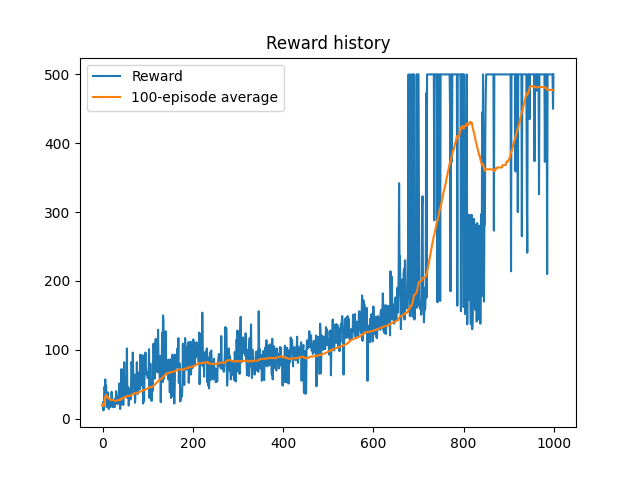
\includegraphics[width=0.9\linewidth]{exercise-5/plots/task-2a.png}
     \caption{Using exponentially decaying variance}
     \label{fig:task-2-a}
   \end{minipage}\hfill
   \begin{minipage}{0.50\textwidth}
     \centering
     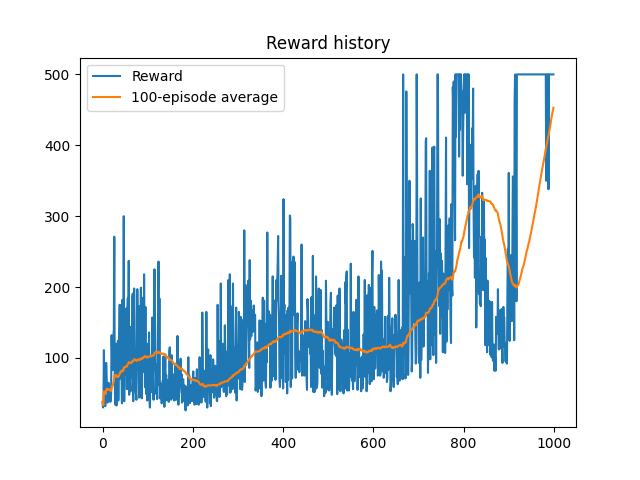
\includegraphics[width=0.9\linewidth]{exercise-5/plots/task-2b.png}
     \caption{Using learnt variance.}
     \label{fig:task-2-b}
   \end{minipage}
\end{figure}

\subsection{Question 3.1}
\textbf{Compare using a constant variance, as in Task 1, to using exponentially decaying variance and to learning variance during training.}\\

When using constant variance, the created distribution for choosing the action that the agent is going to perform has always the same variance, so the probability of choosing actions, starting from the average is always going to be the same. The main advantage of this is that the model always explores more actions, due to the variability of the possible samples, but have the disadvantage that the model does not intensify with less variance.\\

On the other hand, the exponentially decay and learned variance are better options, because they are intensifying the the possible values of the samples, when having more iterations. The main disadvantage of it is that they are computationally more expensive, especially the learnt param, which have to be optimized using the stochastic descent.

\subsection{Question 3.2}
\textbf{In case of learned variance, what’s the impact of initialization on the training performance?}\\

The initialization plays a key role in the performance of training, because the initial value is going to be the one used in the early stages of the training. In case an small value is used, then the model could not find enough exploration range, which is crucial in the beginning. On the contrary, if a value is too big, then the model is going to find difficult to reduce the value and intensify the search of actions in the later stages.

\subsection{Question 4.1}
\textbf{Could the method implemented in this exercise be directly used with experience replay? Why/why not?}\\

We can not use experience replay directly, because the REINFORCE algorithm that we have implemented is off-policy, and experience replay requires an on-policy algorithm that updates the network with each iteration, not with each episode.

\subsection{Question 4.2}
\textbf{Which steps of the algorithm would be problematic to perform with experience replay, if any?}\\

The most problematic step could be the calculation of the best action in the situation, because in the case of REINFORCE is the policy the neural network that gives as an output the distribution of the action to take. On the contrary, in the experience replay algorithm implemented in exercise 4, there were different estimators for the possible actions.

\subsection{Question 5.1}
\textbf{What could go wrong when a model with an unbounded continuous action space and a reward function like the one used here (+1 for survival) were to be used with a physical system?}\\

The main problem there could be the physical restrictions that a machine has but our model does not take into consideration. For example the size of the base of the physical cart pole is limited, so if the agent tries to go to a certain place it could reach the limit and find the physical restriction.

\subsection{Question 5.2}
\textbf{How could the problems appearing in Question 5.1 be mitigated without putting a hard limit on the actions?}\\

One possible solution could be to modify the reward function, in a way that when the agent moves far from the center of the base, the rewards decreases proportionally. This lead the agent eventually learning that when it stays in the center of the pole it receives more rewards.

\subsection{Question 6}
\textbf{Can policy gradient methods be used with discrete action spaces? Why/why not? Which steps of the algorithm would be problematic to perform, if any? }\\

Policy gradient methods are not originally developed for discrete action spaces, nevertheless they could be used with them. One modification that could be done to policy gradient methods could be to use a discrete distribution (such as Bernouilli distribution) instead of a normal distribution in order to select the best action from the policy. \\

There could be problems computing the reward values for discrete action spaces when they became computationally heavy. This is because the standard use are algorithms based on value-function optimization, such as Deep Q-Learning instead of policy gradient for problems with continuous action spaces.

\bibliographystyle{ieeetr}
\bibliography{bibliography}  % Modify template with your bibliography name
\end{document}
